\documentclass[tikz,border=12pt]{standalone}
\usepackage[T1]{fontenc}
\usepackage{lmodern}
\usetikzlibrary{arrows.meta,shapes.geometric}
\tikzset{
  >={Latex[length=2.2mm]},
  every path/.style={line width=.7pt},
  state/.style={draw,line width=1pt,minimum width=4.2cm,minimum height=1cm,font=\small},
  dec/.style={draw,diamond,aspect=2.6,inner sep=1pt,font=\small},
  cond/.style={draw,rounded corners=.5cm,minimum width=3.6cm,minimum height=1cm,font=\small},
  sname/.style={font=\sffamily\bfseries,anchor=south west,inner sep=1pt},
  code/.style={font=\ttfamily\footnotesize,anchor=south east,inner sep=1pt},
  lab/.style={font=\footnotesize,inner sep=1.5pt},
  dot/.style={circle,fill,inner sep=1.4pt}
}
\begin{document}
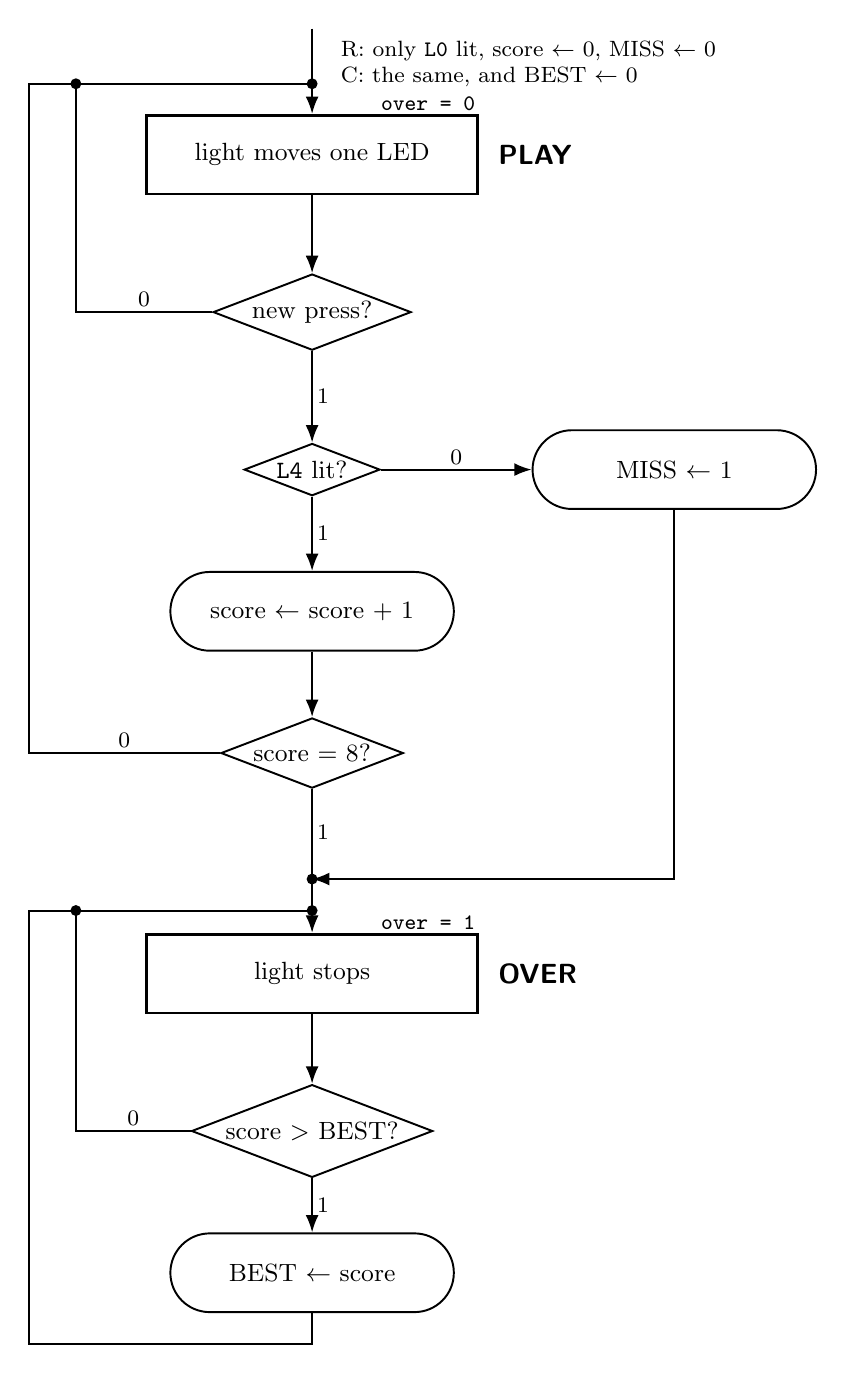
\begin{tikzpicture}
  \node[state] (play) at (0,0) {light moves one LED};
  \node[sname,anchor=west] at ([xshift=2mm]play.east) {PLAY};
  \node[code] at (play.north east) {over = 0};
  \node[dec] (press) at (0,-2.0) {new press?};
  \node[dec] (l4) at (0,-4.0) {\texttt{L4} lit?};
  \node[cond] (inc) at (0,-5.8) {score $\leftarrow$ score + 1};
  \node[dec] (nine) at (0,-7.6) {score = 8?};
  \node[cond] (miss) at (4.6,-4.0) {MISS $\leftarrow$ 1};
  \node[state] (over) at (0,-10.4) {light stops};
  \node[sname,anchor=west] at ([xshift=2mm]over.east) {OVER};
  \node[code] at (over.north east) {over = 1};
  \node[dec] (gt) at (0,-12.4) {score $>$ BEST?};
  \node[cond] (best) at (0,-14.2) {BEST $\leftarrow$ score};

  \draw[->] (0,1.6) -- (play.north);
  \node[lab,anchor=west,align=left] at (0.3,1.15) {R: only \texttt{L0} lit, score $\leftarrow$ 0, MISS $\leftarrow$ 0\\C: the same, and BEST $\leftarrow$ 0};
  \draw[->] (play) -- (press);
  \draw[->] (press) -- node[lab,right] {1} (l4);
  \draw[->] (l4) -- node[lab,right] {1} (inc);
  \draw[->] (inc) -- (nine);
  \draw[->] (l4.east) -- node[lab,above] {0} (miss.west);
  \draw[->] (nine.south) -- node[lab,right,pos=.3] {1} (over.north);
  \draw[->] (miss.south) |- (0,-9.2);
  \node[dot] at (0,-9.2) {};

  \draw (press.west) -- node[lab,above] {0} (-3.0,-2.0) |- (0,0.9);
  \draw (nine.west) -- node[lab,above] {0} (-3.6,-7.6) |- (-3.0,0.9);
  \node[dot] at (0,0.9) {};
  \node[dot] at (-3.0,0.9) {};

  \draw[->] (gt) -- node[lab,right] {1} (best);
  \draw[->] (over) -- (gt);
  \draw (gt.west) -- node[lab,above] {0} (-3.0,-12.4) |- (0,-9.6);
  \draw (best.south) -- (0,-15.1) -| (-3.6,-9.6) -- (-3.0,-9.6);
  \node[dot] at (0,-9.6) {};
  \node[dot] at (-3.0,-9.6) {};
\end{tikzpicture}
\end{document}
